\section{Introduce}

%------------------------------------------------
\begin{frame}[fragile]{ RS485 feature}

\begin{itemize}
\item  485 is  Fully balanced
\item 485 handles multiple drivers and receivers
\item Better common-mode noise rejection (-7 to +12Volts)
\item Sensitivity of 200mV in receivers
\item Drivers give up to 5 volts balanced output
\item Can stand contention, driver shuts down by itself
\item High input resistance (12K ohms)
\item Hysteresis of 50 mv to overcome diff. noise
\end{itemize}

\begin{figure}[htbp]
\begin{center}
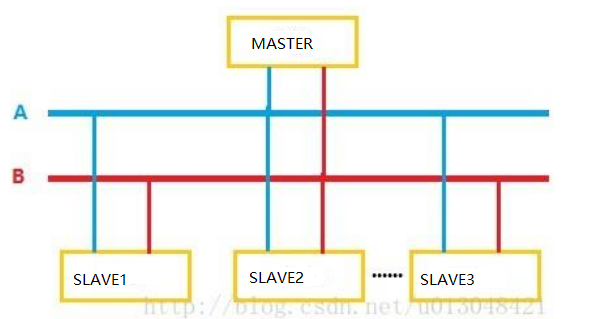
\includegraphics[width=5cm]{img/485net}
\caption{485NET }
\label{Overview}
\end{center}
\vspace{-0.5em}
\end{figure}

\end{frame}


%------------------------------------------------
\begin{frame}[fragile]{The Principle of The BAN's Clock Synchronization}

\begin{itemize}
  \item In order to synchronize the device clock, it is necessary to add a clock line between Master and Slave, where Master generates synchronous clock square wave.
\end{itemize}

\begin{figure}[htbp]
\begin{center}
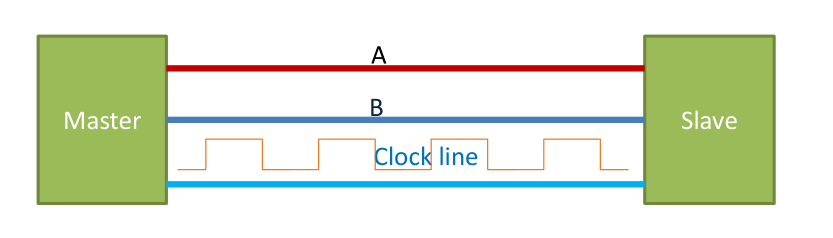
\includegraphics[width=6cm]{img/syncchart}
\caption{synchronous}
\label{Overview}
\end{center}
\vspace{-0.5em}
\end{figure}
\end{frame}


%------------------------------------------------
\begin{frame}[fragile]{Our Design}
We designed it like this:
\begin{figure}[htbp]
\begin{center}
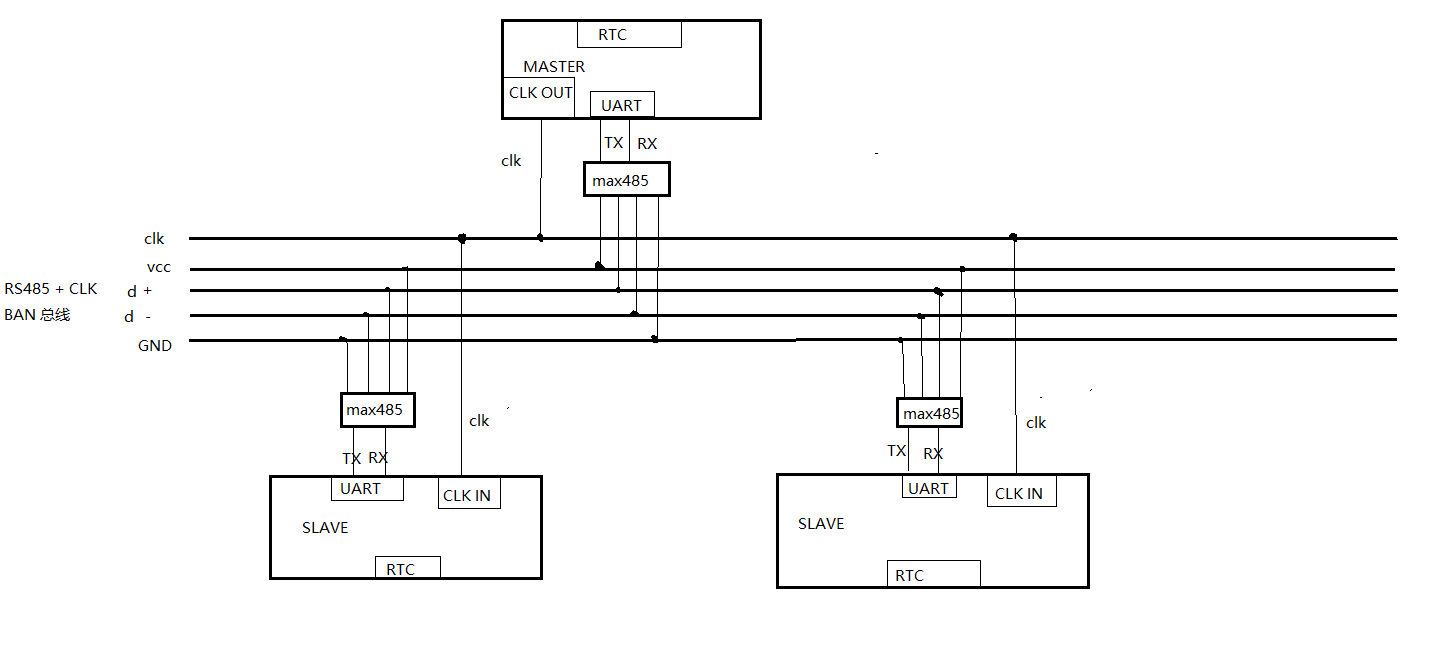
\includegraphics[width=10cm]{img/overview}
\caption{BAN }
\label{Overview}
\end{center}
\vspace{-0.5em}
\end{figure}
\end{frame}





%------------------------------------------------
\begin{frame}[fragile]{BUS}

\begin{enumerate}
\item Adding a clock line from RS485 to form the basic hardware circuit of BAN bus.
\item The clock  line is used to generate Millisecond-level pulses for clock synchronization.Later aliases:SYNC\_CLK
\item D +, D - is  differential  signal  .

\end{enumerate}

we assumed that the device mounted on the bus has one Master and two Slaves.


\end{frame}

%------------------------------------------------
\begin{frame}[fragile]{Local Clock Counter \& SYNC\_CLK}

\begin{itemize}
\item  Local Clock Counter , Each device has a local clock counter. The timing granularity is 100us.

\item  SYNC\_CLK,The device on BAN bus uses clock line to complete clock synchronization. Master's timer generates synchronization pulse, Slave'scaptures synchronized  pulse to complete synchronization.
\end{itemize}


\end{frame}





%------------------------------------------------
\begin{frame}[fragile]{Synchronization process}

\begin{itemize}
\item a. master and slave power on and initialize peripherals.
\item b. master starts sending square wave signals,at The first rising edge of
square wave signal:
  \begin{enumerate}
    \item  The master starts Master's Local Clock Counter(MLCC).
    \item Slave captures this rising edge at the same time.Then start Slave's Local Clock Counter(SLCC).
    \item The delay of the rising edge of the clock line transmission can be neglected, So we think that MLCC and SLCC start counting at the same time.
  \end{enumerate}
 \item c. Slave calibrates SLCC at each subsequent SYNC\_CLK rising edge.

\end{itemize}



\begin{figure}[htbp]
\begin{center}
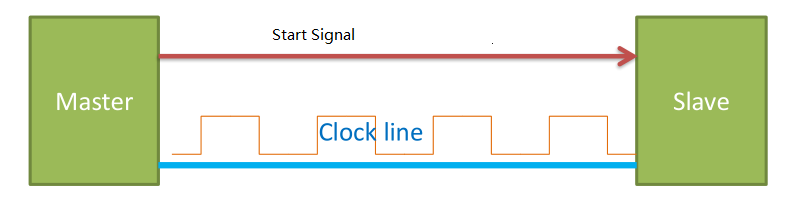
\includegraphics[width=6cm]{img/abstim}
\caption{BAN }
\label{Overview}
\end{center}
\vspace{-0.5em}
\end{figure}
\end{frame}





%------------------------------------------------
\begin{frame}[fragile]{Clock Difference Calibration}

SYNC\_CLK is produced by Master with fixed period and precise time.Let's take a period of 16 milliseconds for example.

MLLC and SLLC start counter at the sametime(first SYNC\_CLK rising edge). Their timing granularity is small, 100 microseconds.

So when the system runs, there are two counts on each device, the Local Clock Count(Every 100 microseconds plus 1) and the SYNC\_CLK Count(Every 16 milliseconds plus 160).Slave calibrates SLCC at each subsequent SYNC\_CLK rising edge by Make those two counts the same.



\end{frame}




%------------------------------------------------
\begin{frame}[fragile]{Clock Difference Calibration}

  \begin{figure}[htbp]
  \begin{center}
  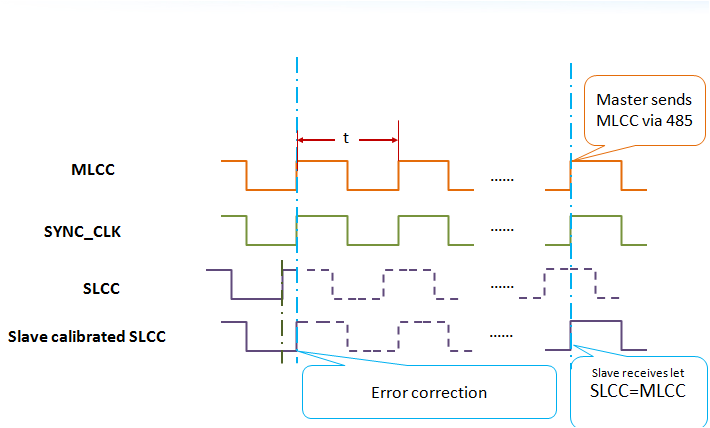
\includegraphics[width=10cm]{img/flow}
  \caption{BAN }
  \label{Overview}
  \end{center}
  \vspace{-0.5em}
  \end{figure}

\end{frame}






%------------------------------------------------
\begin{frame}[fragile]{Demo implementation}

The following is the demo wiring and structure:
\begin{figure}[htbp]
\begin{center}
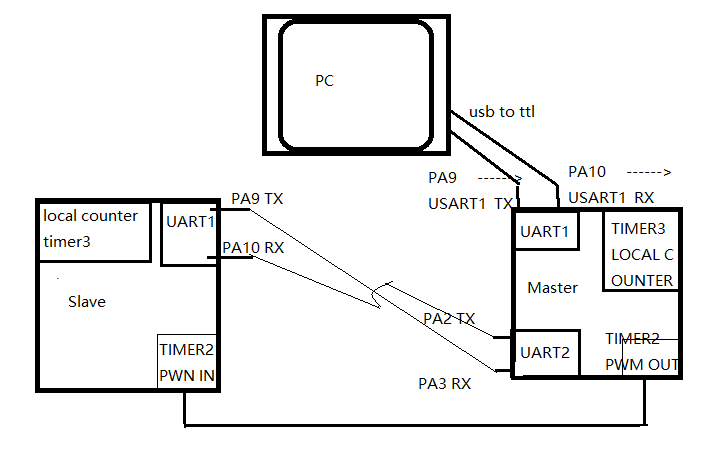
\includegraphics[width=10cm]{img/demo0}
\caption{demo}
\label{Overview}
\end{center}
\vspace{-0.5em}
\end{figure}

\end{frame}
